
\begin{figure}[t]
\begin{centering}
    {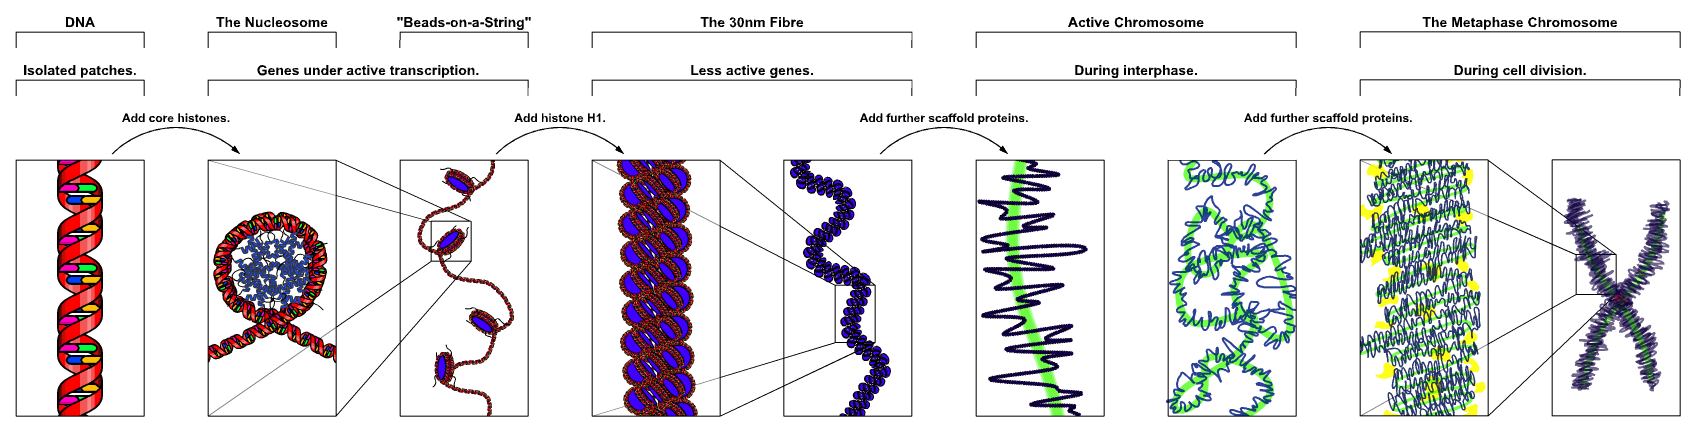
\includegraphics[scale=0.25]{figures/background/Chromatin_Structures}}
    \caption[Major Chromatin Structures]
    {\textbf{Major Chromatin Structures.}

    Note that the rightmost structures are only found during cell division, the
    cell is in interphase during most of the time. \\ \\ Image from \cite{figChromatinStructures}.}
    \label{fig:comparison3C}\label{fig:chromatin}
\end{centering}
\end{figure}



